\subsection{Resistive and Capacitive load}

\subsubsection{Adjusted boundary conditions}

Adding a capacitance in parallel with the load as depicted in figure \ref{fig:Rl_Cl} gives rise to some adjustements to the voltage update function at $z=0$.

\begin{figure}
    \centering
    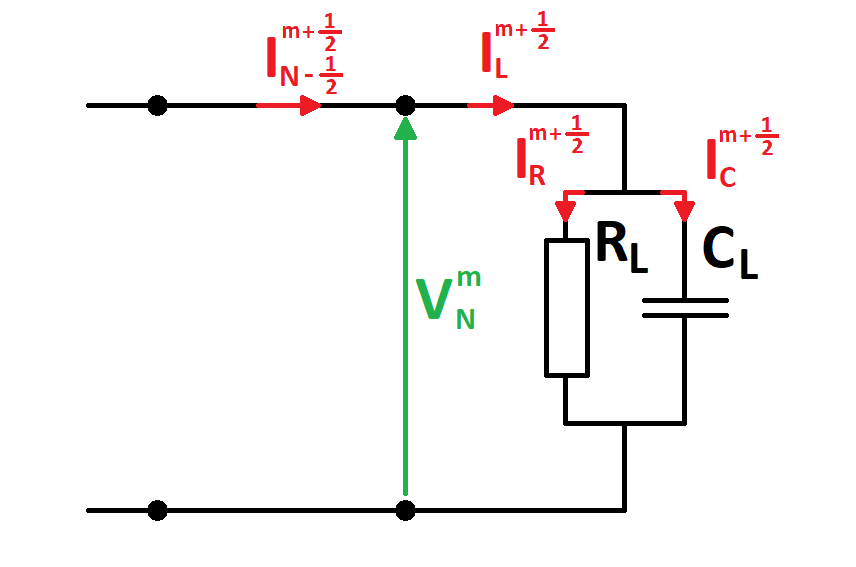
\includegraphics[scale=0.35]{BC2_cap}
    \caption{Load with capacitance}
    \label{fig:Rl_Cl}
\end{figure}

Kirchoff's current law states now that
\begin{equation}
    I^{m+\frac{1}{2}}_{L} = I^{m+\frac{1}{2}}_{R} + I^{m+\frac{1}{2}}_{C}.
    \label{IL2}
\end{equation}
Using Kirchoff's voltage law at the resistor gives
\begin{align}
    I^{m+\frac{1}{2}}_{R} & = \frac{V^{m+\frac{1}{2}}_{N}}{R_{L}}\nonumber\\
    & = \frac{V^{m}_{N}+V^{m+1}_{N}}{2R_{L}}
    \label{IR}
\end{align}
The relation between the current and the voltage at the capitor is given by
\begin{equation}
    \hat{i} = C\frac{\partial \hat{v}}{\partial t}.
\end{equation}
For a first order FDM this turns into
\begin{equation}
    I^{m+\frac{1}{2}}_{C} = C_{L}\frac{V^{m+1}_{N} - V^{m}_{N}}{\Delta t}.
    \label{IC}
\end{equation}
Substituting (\ref{IR}) and (\ref{IC}) into (\ref{IL2}) gives
\begin{equation}
    I^{m+\frac{1}{2}}_{L} = \left(\frac{1}{2R_{L}}+\frac{C_{L}}{\Delta t}\right)V^{m+1}_N + \left(\frac{1}{2R_{L}}-\frac{C_{L}}{\Delta t}\right)V^{m}_N
\end{equation}
and can be rewritten as
\begin{equation}
    \tilde{I}^{m+\frac{1}{2}}_{L} = \frac{R_{c}}{2Z_{2}}V^{m+1}_N + \frac{R_{c}}{2Z_{1}}V^{m}_N
    \label{IL2_final}
\end{equation}
with
\begin{align}
    Z_{1} &= \left(\frac{1}{R_{L}}-2\frac{C_{L}}{\Delta t}\right)^{-1} = \frac{R_{L}\Delta t}{\Delta t - 2 C_{L}R_{L}} \nonumber\\
    Z_{2} &= \left(\frac{1}{R_{L}}+2\frac{C_{L}}{\Delta t}\right)^{-1} = \frac{R_{L}\Delta t}{\Delta t + 2 C_{L}R_{L}} \label{eq:Z}
\end{align}
Substituting (\ref{IL2_final}) into the adjusted voltage update function at $z=d$ yields
\begin{equation}
    V^{m+1}_{N} = K'_{2}V^{m}_N + 2\kappa'_{2}\tilde{I}^{m+\frac{1}{2}}_{N-\frac{1}{2}},
\end{equation}
where
\begin{align}
    K'_{2} & = \frac{Z_{2}}{Z_{1}}\frac{Z_{1}-\alpha R_{c}}{Z_{2}+\alpha R_{c}},\\
    \kappa'_{2} & = \frac{\alpha Z_{2}}{Z_{2}+\alpha R_{c}}.
\end{align}
are the new dimensionless constants.

\subsubsection{Influence of C}

First thing to notice is that when $C_{L} = 0$ then $K'_{2} = K_{2}$ and $\kappa'_{2} = \kappa_{2}$. This is a good
sign since it stays consistent with the previous update equation.\\
Secondly in relations \ref{eq:Z} there is a time step dependecy, hence the two dimensionless
coefficients in the boundary update function at $z=d$ are also dependent on the implemented time step. Let's consider a
well chosen time step and just look at the effect of changing $C_{L}$.
\begin{itemize}
    \item $C_{L} \rightarrow 0$ :
        $K'_{2} \rightarrow K_{2}$ and $\kappa'_{2} \rightarrow \kappa_{2}$, initial situation
    \item $C_{L} \rightarrow \infty$ :
        $ K'_{2} \rightarrow 1$ and $\kappa'_{2} \rightarrow 0$, fully reflected wave
    \item $C_{L} \rightarrow \frac{\Delta t}{2R_{L}}$ :
        $K'_{2} \rightarrow \frac{Z_{2}}{Z_{2}+\alpha R_{C}}$ and $\kappa'_{2} \rightarrow \frac{2\alpha Z_{2}}{Z_{2}+\alpha R_{C}}$, this shows that the division by zero for $Z_1$ does not lead to any problems.
\end{itemize}

\begin{figure}[H]
    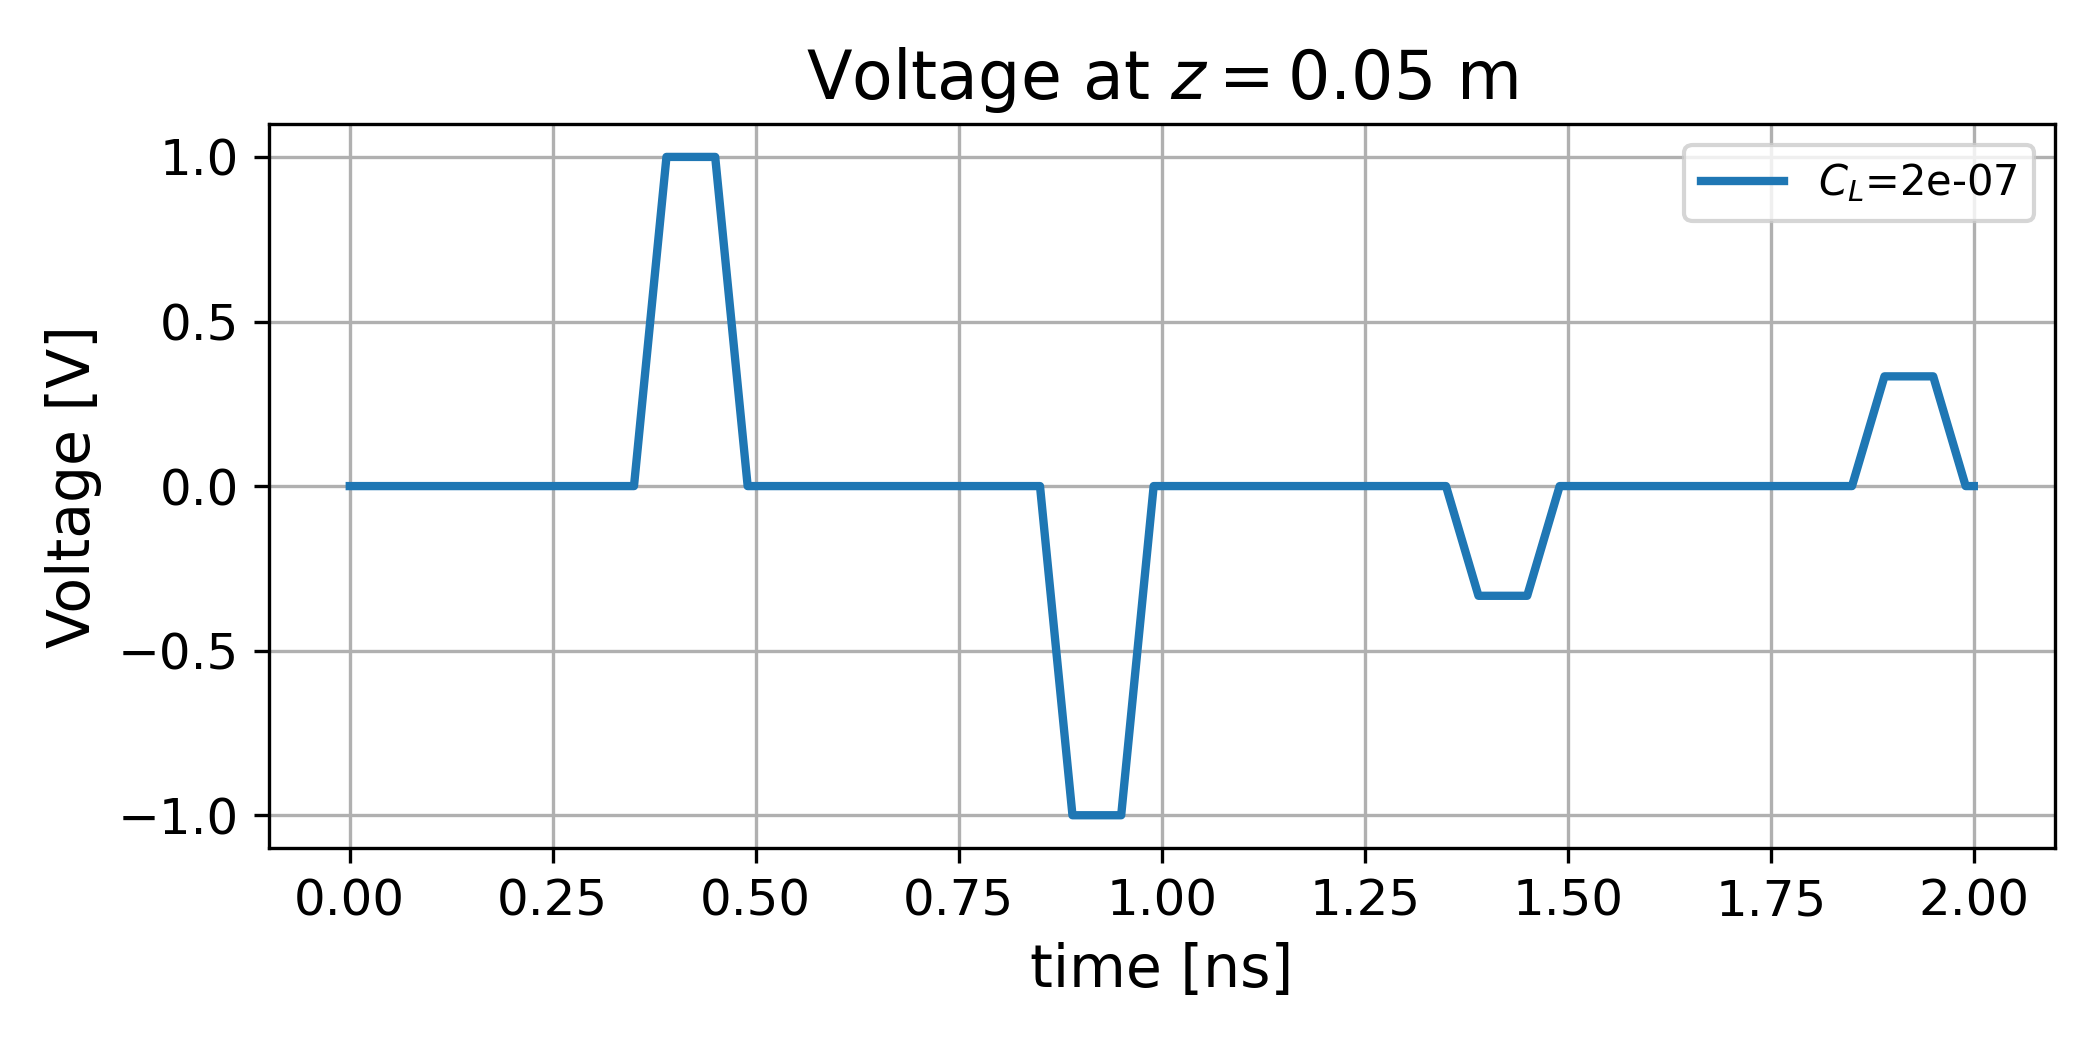
\includegraphics[scale=0.5]{example_C=2e-07_time.png}
    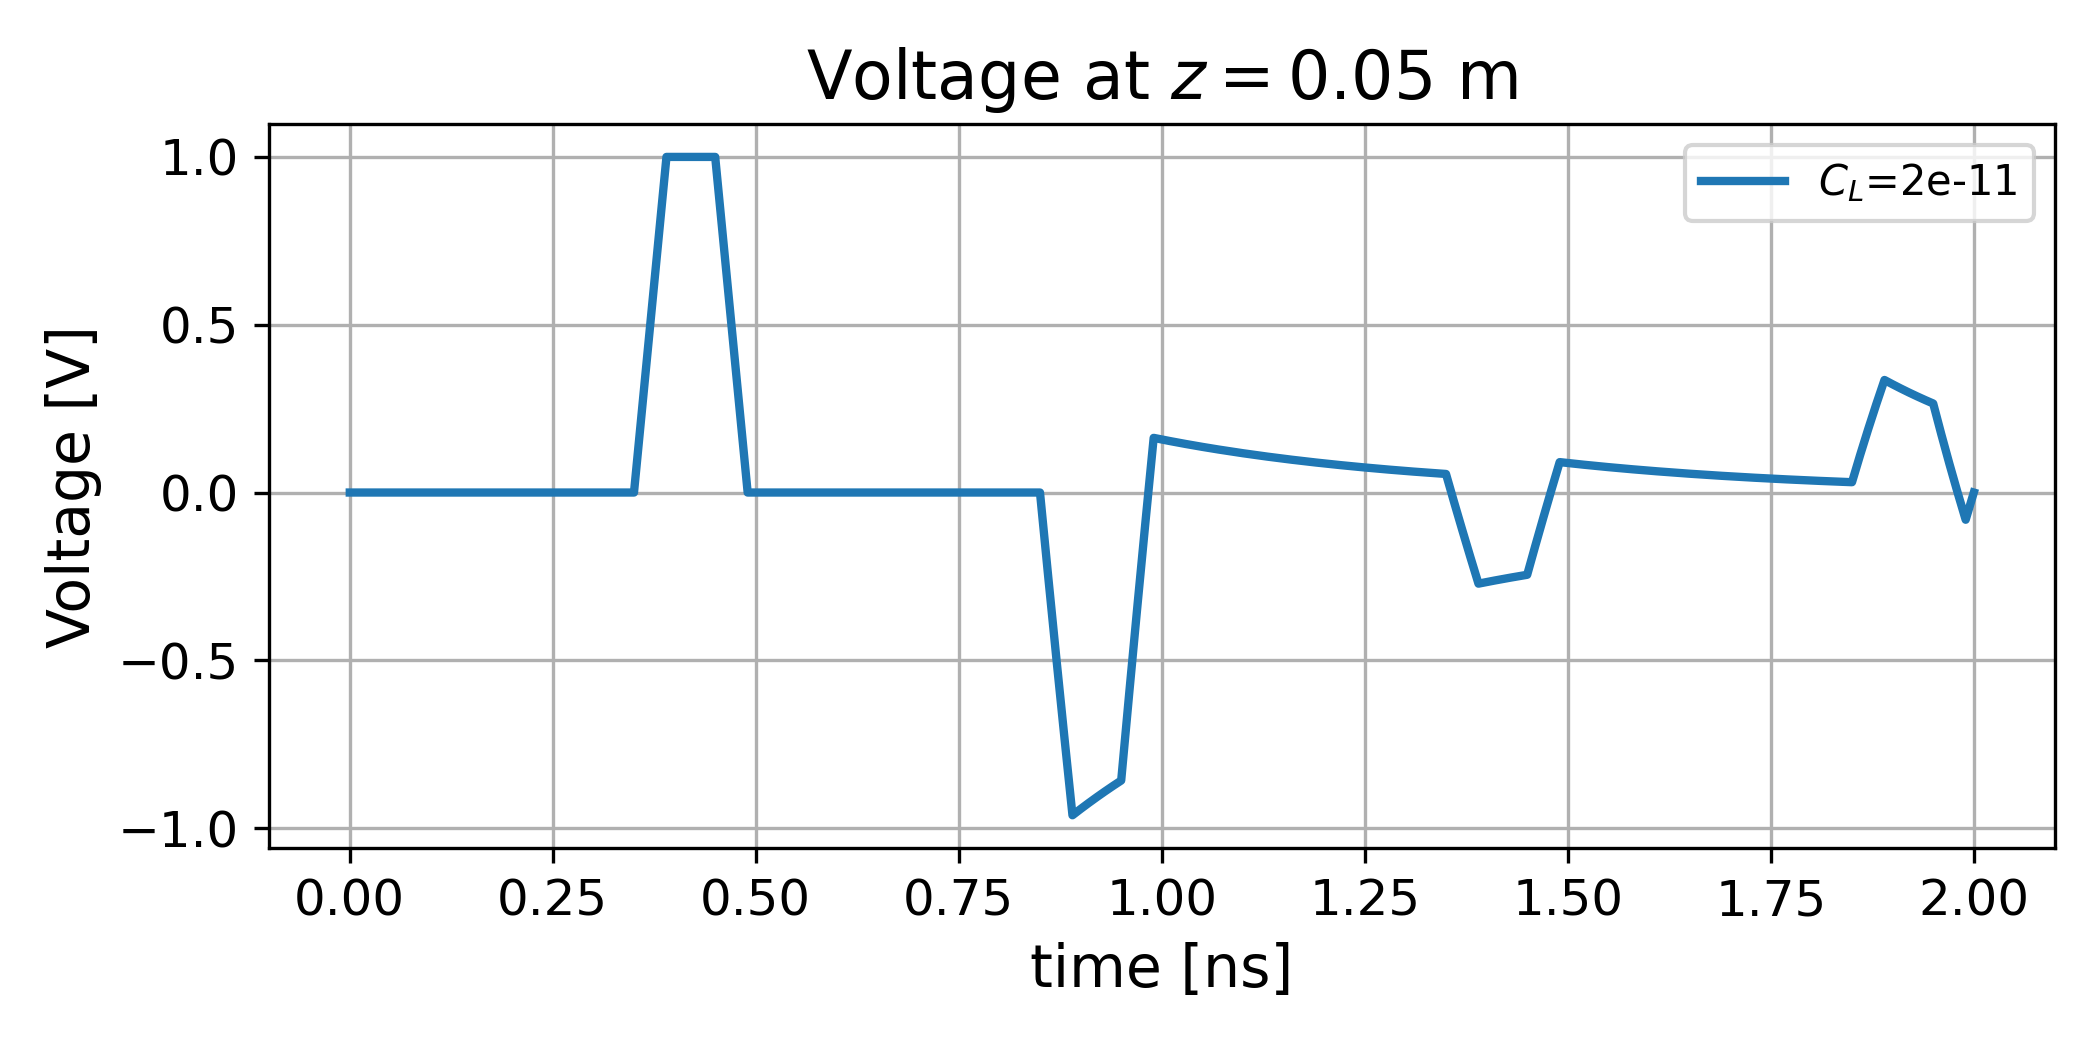
\includegraphics[scale=0.16]{example_C=2e-11_time.png}

    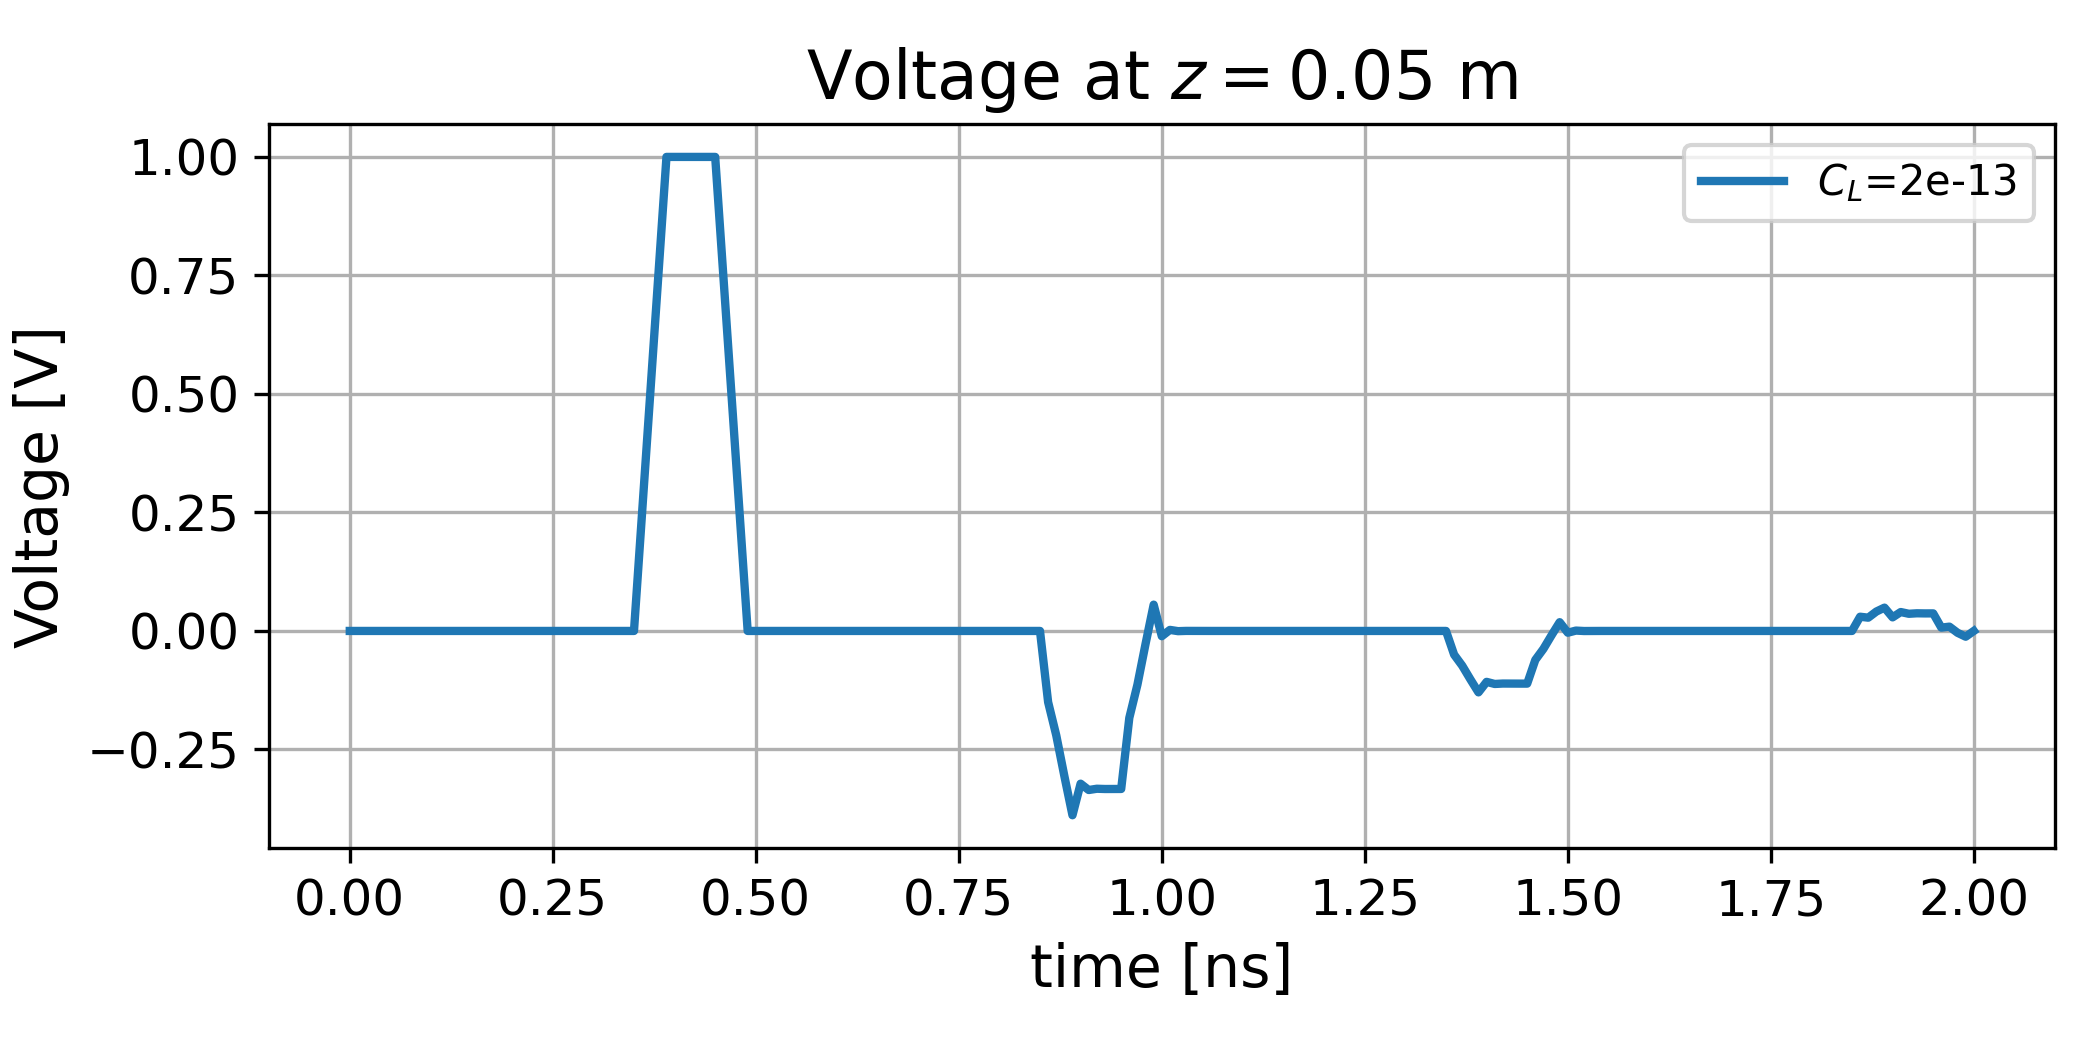
\includegraphics[scale=0.5]{example_C=2e-13_time.png}
    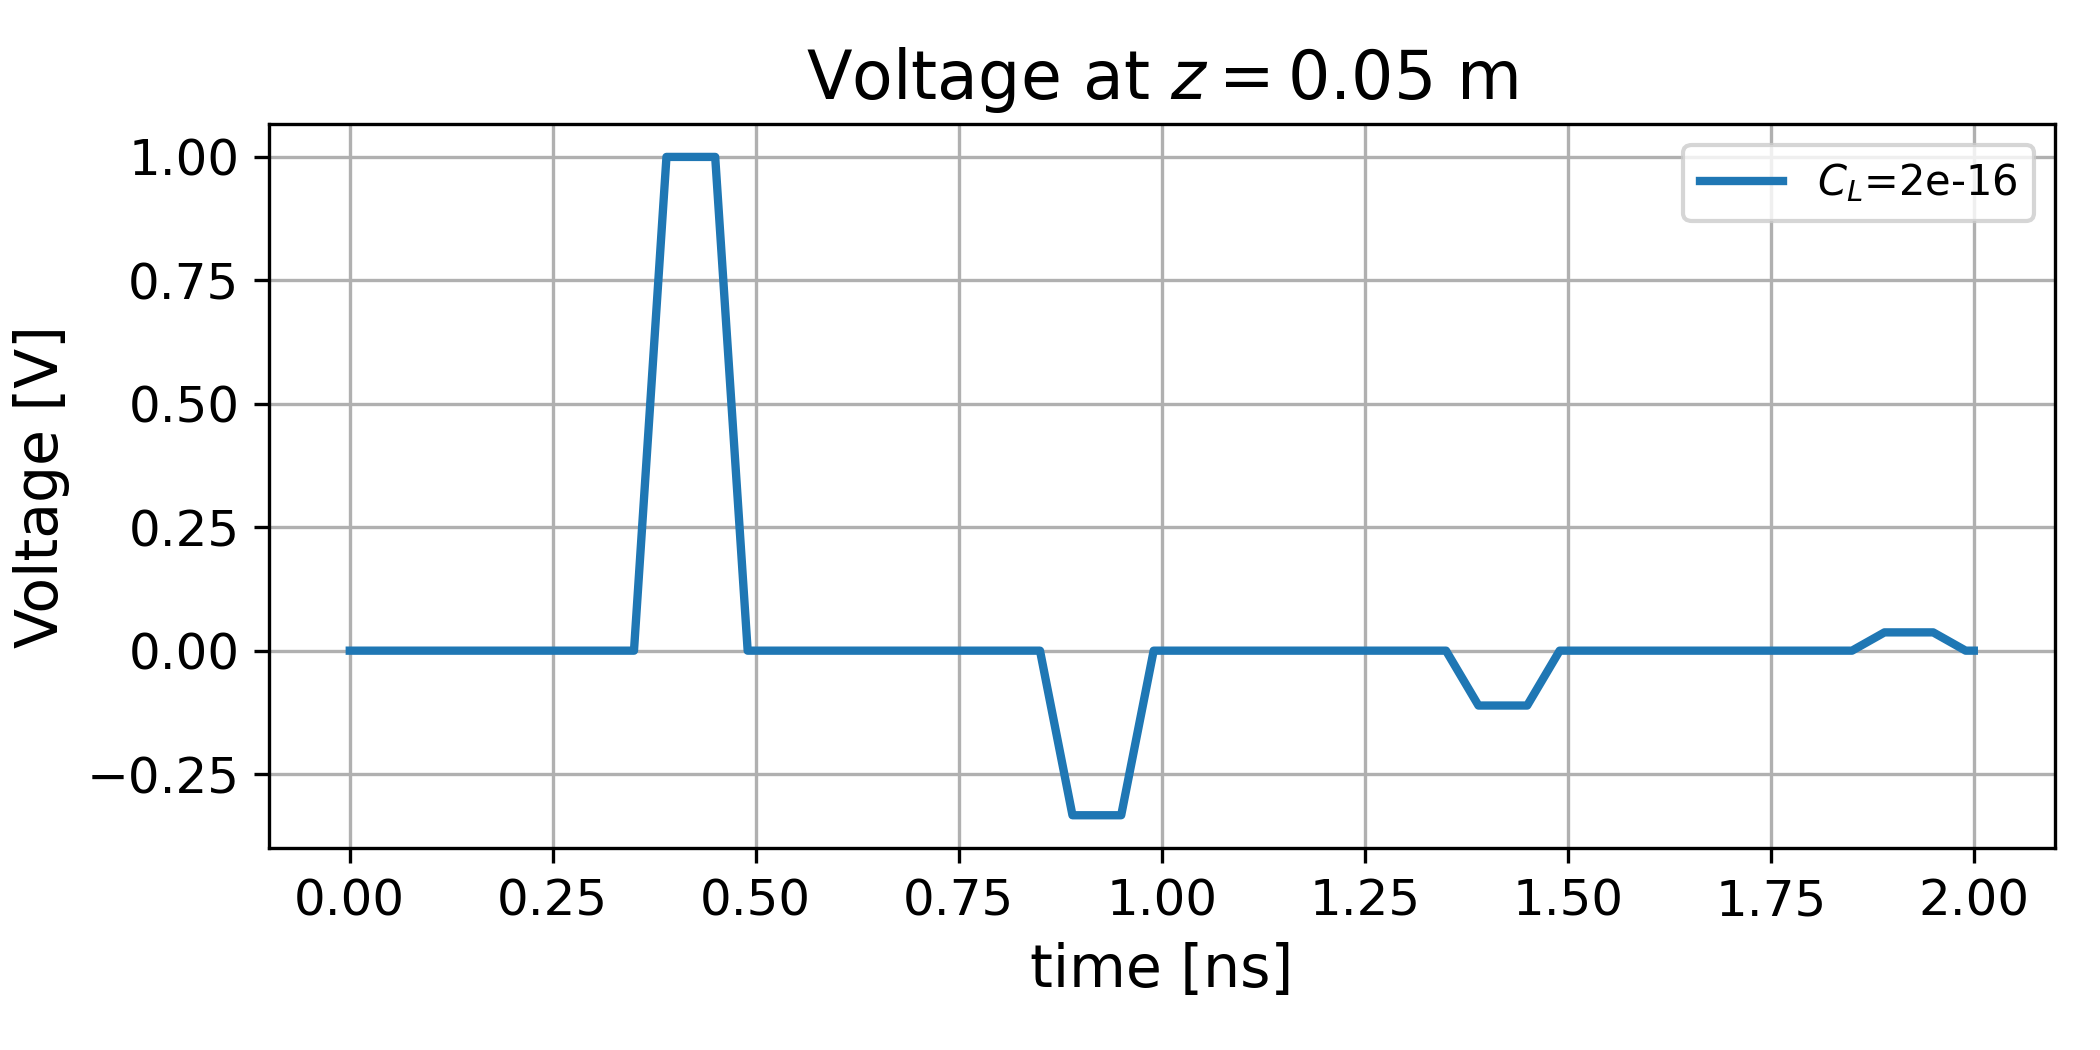
\includegraphics[scale=0.5]{example_C=2e-16_time.png}
    \caption{Different values for the load capacitance}
    \label{fig:effect_CL}
\end{figure}

From figure \ref*{fig:effect_CL} the following obesrvations can be made:
\begin{itemize}
    \item For large values of the capacitance no energy loss will occur at the load, i.e. the amplitude of the voltage does not change when passing the load. The capacitor has enough capacitance to store the whole bit and return it to the transmision line.
    \item For intermediate values for the capacitance, i.e. $C_L = 2e-11$, the decharging of the capacitor can clearly be seen (exponetial drop).
    \item When the capacitance gets very low its effect gets negligible.
\end{itemize}